\documentclass[11pt]{article}
\usepackage[a4paper,margin=1in]{geometry}
\usepackage{graphicx}
\usepackage{amsmath,amssymb}
\usepackage{booktabs}
\usepackage{hyperref}
\usepackage{xcolor}
\usepackage{caption}

\IfFileExists{generated/run_numbers.tex}{\input{generated/run_numbers.tex}}{%
\newcommand{\SelectedSources}{492}
\newcommand{\EquationWitnesses}{1408}
\newcommand{\UsableMechanisms}{204}
\newcommand{\CaseMechanisms}{72}
\newcommand{\EvidenceGradeMechanisms}{35}
\newcommand{\DirectSafetyMechanisms}{0}
\newcommand{\AstroAnalogues}{28}
\newcommand{\ThresholdHooks}{1}
\newcommand{\CaseAnalogues}{24}
\newcommand{\CaseTransferAnalogues}{51}
}

\title{A Mechanism-First Audit of the LHC Black-Hole Safety Debate}
\author{Public demo generated from static audit artifacts}
\date{}

\begin{document}
\maketitle

\begin{abstract}
Scientific evidence has two separable graph layers. A provenance graph records who
made a claim, where it appears, and how sources support or challenge one another.
A mechanism graph records something different: which equations instantiate the
physical steps by which a claim could become true. We demonstrate the distinction
on the LHC microscopic-black-hole debate using only static public audit artifacts.
In \SelectedSources{} selected arXiv sources, the strict gate recovered
\EquationWitnesses{} equation witnesses, \UsableMechanisms{} formula-clean
mechanism nodes, \CaseMechanisms{} LHC-black-hole case-relevant nodes, and
\EvidenceGradeMechanisms{} evidence-grade case nodes. The branch split was
asymmetric: \DirectSafetyMechanisms{} source-local formula-clean direct
LHC-safety mechanisms, \ThresholdHooks{} collider-threshold or event-selection
hook, and \AstroAnalogues{} astrophysical black-hole analogues. The substantive
output is therefore not another list of stances. It is a map of which physical
mechanisms are present in the corpus and which translation steps from adjacent
black-hole physics would have to be made explicit.
\end{abstract}

\section{The Problem}

Most automated controversy maps stop at statements: a source said that the collider
is safe, unsafe, misleading, or incomplete. That representation is useful, but it
places all evidence on the same social layer. The LHC black-hole case requires a
different object. The scientific content is the branch structure of the proposed
mechanism:
\[
\begin{aligned}
\mathrm{production} &\rightarrow \mathrm{evaporation\ or\ stability}
\rightarrow \mathrm{capture/stopping}\\
&\rightarrow \mathrm{accretion/growth}
\rightarrow \mathrm{astrophysical\ bound} .
\end{aligned}
\]
Each arrow is a physical slot that must be filled by equations, observations, or
controlled assumptions. This is why the demo builds two graphs from the same
papers.

\section{Two Graphs in the Same Archive}

\textbf{Provenance graph.} Nodes are sources and claims. Edges record that a
source makes a claim, belongs to a claim family, or supports a stated position.
This graph answers attribution questions: who said what, where, and in relation
to which other sources.

\textbf{Mechanism graph.} Nodes are equation witnesses and local formula
transitions. Edges record source-local route transitions and cross-source route
analogues. A node is evidence-grade only if the local formula window contains
both the black-hole case and a mechanism category. Source-level words alone are
not enough. In this report, ``formula-clean'' means that the extracted local
window survived the equation-quality gate and retained a recognizable mathematical
relation, not just prose or bibliographic residue.

\begin{figure}[t]
\centering
\IfFileExists{figures/provenance_vs_mechanism.pdf}{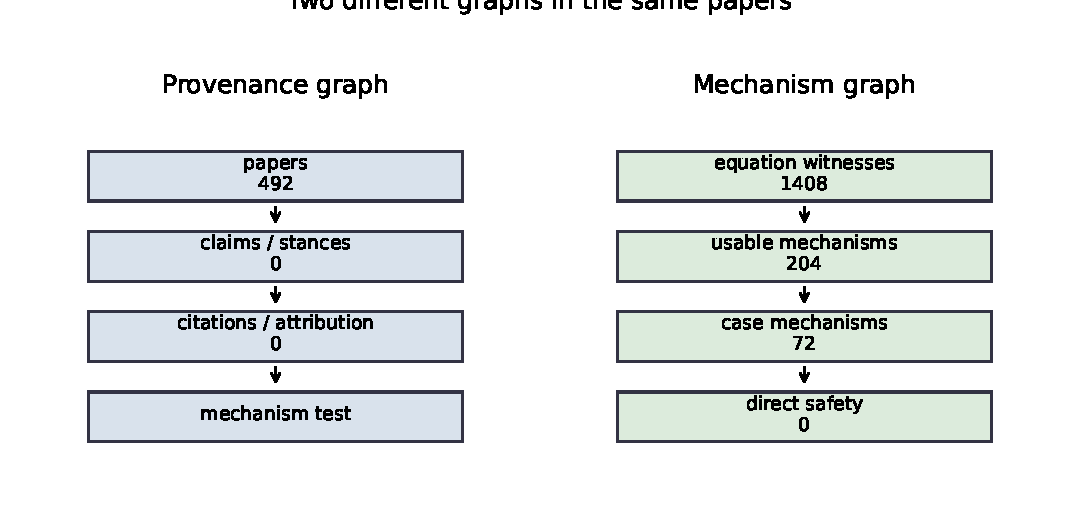
\includegraphics[width=0.92\linewidth]{figures/provenance_vs_mechanism.pdf}}{\fbox{Missing figure: provenance\_vs\_mechanism.pdf}}
\caption{A provenance graph and a mechanism graph answer different questions. The first organizes attribution. The second records whether equation-level mechanisms are present and whether they can be translated between branches.}
\end{figure}

\section{Mechanism Gates}

The mechanism graph uses six route labels as an interface to equation
transformations. The labels are deliberately coarse: they are gates for audit,
not names for complete theories.
\[
\begin{array}{ll}
\text{transport/flow} & \partial_t q + \nabla\cdot J = S,\\
\text{constraint/closure} & C(q,J,\lambda)=0,\\
\text{spectral/operator} & Lq=\lambda q,\\
\text{boundary/weak form} & \int_\Omega \phi Lq=\int_\Omega \phi f,\quad Bq=b,\\
\text{commutator/residual} & [A,B]=AB-BA,\\
\text{discrete protocol} & x_{n+1}=\Phi(x_n,u_n).
\end{array}
\]
A receipt is a local equation witness that activates one or more of these gates
inside a case-relevant formula window. This makes the audit stricter than keyword
search but more inspectable than an uninterpreted embedding.

\section{Results}

\begin{figure}[t]
\centering
\IfFileExists{figures/evidence_funnel.pdf}{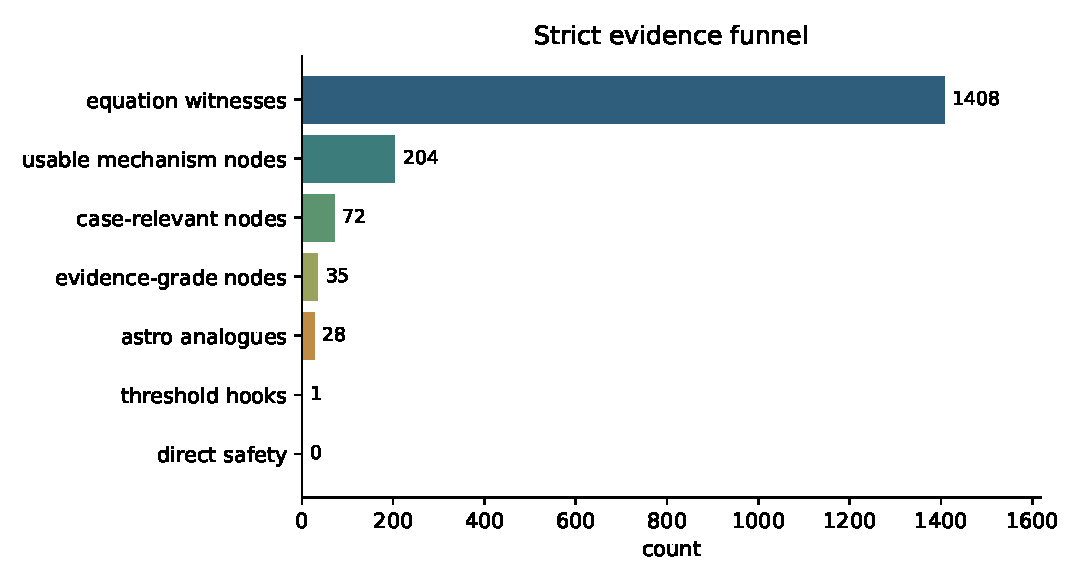
\includegraphics[width=0.86\linewidth]{figures/evidence_funnel.pdf}}{\fbox{Missing figure: evidence\_funnel.pdf}}
\caption{Strict evidence funnel. Most extracted witnesses are rejected or kept only as audit material. The public result is the branch split: no direct safety mechanism under the gate, one threshold hook, and many adjacent astrophysical mechanisms.}
\end{figure}

The strict run gives the following public counts:
\[
\begin{array}{lr}
\text{equation witnesses} & \EquationWitnesses\\
\text{usable formula-clean mechanism nodes} & \UsableMechanisms\\
\text{case-relevant nodes} & \CaseMechanisms\\
\text{evidence-grade case nodes} & \EvidenceGradeMechanisms\\
\text{direct LHC-safety mechanisms} & \DirectSafetyMechanisms\\
\text{collider-threshold hooks} & \ThresholdHooks\\
\text{astrophysical black-hole analogues} & \AstroAnalogues.
\end{array}
\]

The result is precise within the selected corpus and gate definition. Direct
source-local LHC-safety equations did not survive the strict evidence gate.
Adjacent black-hole physics did: accretion, evaporation, capture, mass growth and
compact-object survival. The scientific task exposed by the graph is therefore a
translation problem: which adjacent mechanisms can be carried into the collider
branch, and what assumptions are required for that transfer?

\section{Mechanism Translation to the LHC Branch}

The equations below state the slots that the audit tries to fill. A collider
branch first needs a production or event-selection condition, for example
\[
\sqrt{s} > M_D ,
\]
followed by a branch decision. If evaporation dominates, the relevant local
receipt should support a mass-loss inequality or lifetime ordering such as
\[
\frac{dM}{dt} < 0,\qquad \tau_{\rm evap}\ll \tau_{\rm capture}.
\]
If a stable object is assumed, the mechanism changes to stopping, capture and
growth:
\[
\frac{dM}{dt} = \rho\,\sigma(M)\,v .
\]
Astrophysical survival bounds then become external tests on the same mechanism.
A dangerous growth branch would have to be compatible with compact-object
observations; schematically,
\[
t_{\rm grow} < t_{\rm WD}
\]
would conflict with the observed survival of white dwarfs if the same production,
capture and growth mechanism were already realized in nature. The graph therefore
does not merely count black-hole papers. It separates the collider threshold,
the evaporation branch, the stable-growth branch and the astrophysical bound.

\begin{figure}[t]
\centering
\IfFileExists{figures/mechanism_translation.pdf}{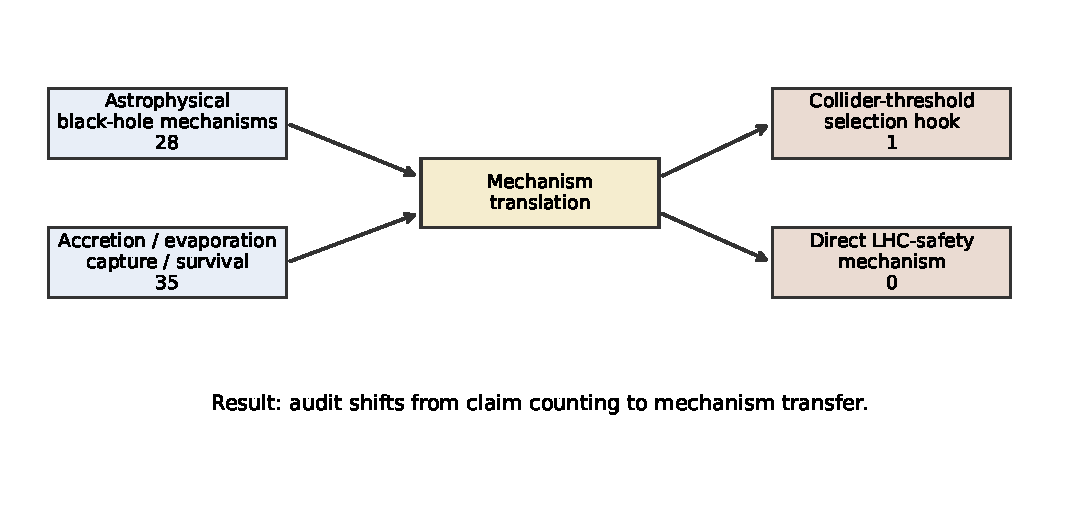
\includegraphics[width=0.92\linewidth]{figures/mechanism_translation.pdf}}{\fbox{Missing figure: mechanism\_translation.pdf}}
\caption{The demo result is a mechanism-translation map. Adjacent black-hole mechanisms provide the inspectable scientific substrate. The collider branch supplies only a threshold hook in this run.}
\end{figure}

\section{Sparse-Attention Support}

The sparse-attention audit reads the static mechanism graph and asks which routes
co-activate in the evidence-grade case layer. It is a consistency check on the
branch split: if the graph is meaningful, adjacent astrophysical receipts should
concentrate in growth, capture, evaporation or boundary-style mechanisms rather
than in direct collider-safety derivations.

\begin{itemize}
\item Sparse-attention receipts are generated when \texttt{sparse\_attention\_audit.json} is available.
\end{itemize}

\begin{figure}[t]
\centering
\IfFileExists{figures/sparse_attention_routes.pdf}{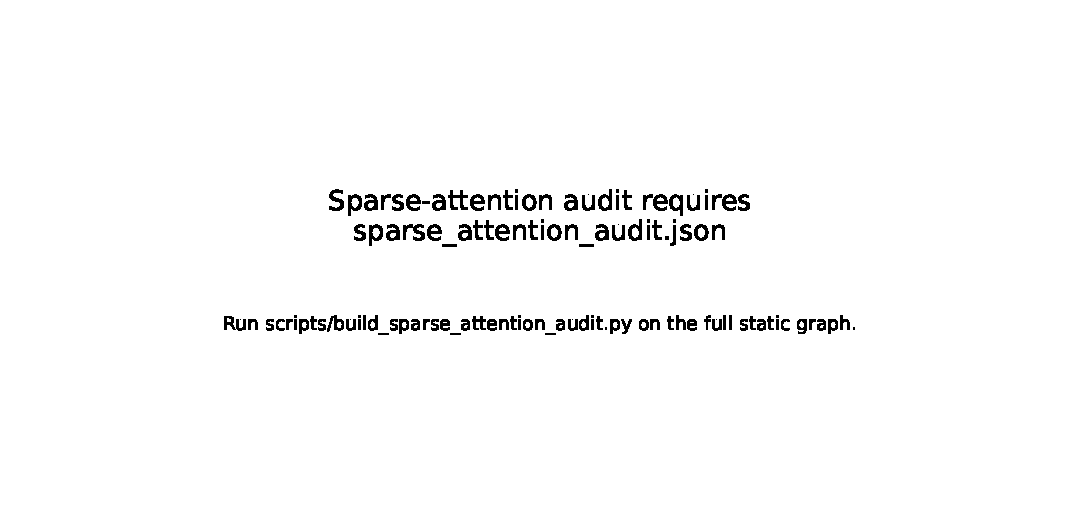
\includegraphics[width=0.92\linewidth]{figures/sparse_attention_routes.pdf}}{\fbox{Missing figure: sparse\_attention\_routes.pdf}}
\caption{Sparse co-activation between case branches and mechanism routes. The important signal is concentration in adjacent astrophysical mechanisms, not direct collider-safety derivations.}
\end{figure}

\section{What the Mechanism Graph Adds}

A provenance-only graph can identify papers, authors, dates and claim families.
It is useful for scrutiny of attribution and incentives. The mechanism graph adds
the missing scientific layer: whether a claimed branch has equation-level support.
In this run, provenance can organize disagreement about LHC safety, but the
mechanism graph explains the structure of the evidence. The direct safety branch
is empty under the strict gate. The adjacent astrophysical branch is populated.
This distinction is not visible from a claim map alone.

\section{Scope and Reproducibility}

The repository is a public audit object built from static outputs. It is designed
to be inspectable without private pipeline files: derived graphs, run summaries,
figures and report text are included; raw fingerprints, model checkpoints and core
pipeline code are not. A complete safety review would extend the same audit to
the full literature search and to non-arXiv safety reports.

\end{document}
